\documentclass{beamer}

% \usepackage{mdframed}
\usepackage[utf8]{inputenc}
\usepackage{default}

\begin{document}



	\title[Crisis]{Secure Two Party Computation}
	\subtitle{Preliminary presentation}
	\author[Author]{Nick Tutte\\[1ex]{\tiny Prof. Nigel Smart}}
	\date[Feb 2015]
	{February, 2015}
	\subject{Computer Science}
	\frame{\titlepage}


	\begin{frame}
		\frametitle{Presentation overview}
		My project focuses on Secure Multiparty Computation, in particular the two party case using Yao Garbled Circuits.\\

		By the end of this presentation you should know,
		\begin{itemize}
			\item What is Secure Multiparty Computation?
			\item What can it be used for?
			\item What ``Secure'' means in this context.
			\item A grounding in Yao Garbled Circuits.
			\item How much progress I've made so far.
		\end{itemize}

	\end{frame}


	\begin{frame}
		\frametitle{What is Secure Multiparty Computation}
		In the problem of Secure Multiparty Computation we have a set of parties, each of whom has a secret input. The parties wish to co-operate to compute a function upon their collective inputs without revealing said inputs.\\
		
		% Diagram here to explain the point.
	\end{frame}


	\begin{frame}
		\frametitle{Applications of Secure Multiparty Computation}
		\begin{itemize}
			\item The Millionaires problem.
			\item Distributed secrets.
			\item Sugar Beets.
			\item Database query.
		\end{itemize}
		
		% Briefly go over each of these applications. Explain what they are. Pictures to fill in the white space?
		For many more potential applications of Secure Multiparty Computation see (Du and Atallah, 2001).
	\end{frame}


	\begin{frame}
		\frametitle{Desired security properties}

		Before we go any further we need to define what properties we want an SMC protocol to fulfil before we consider it Secure.
		
		\begin{itemize}
			\item Privacy, the only knowledge parties gain from participating is the output.
			\item Correctness, the output is indeed that of the intended function.
			\item Independence of inputs, no party can choose it's inputs as the function of other parties inputs.
			\item Fairness, corrupt parties receive their outputs if and only if the honest parties also receive their outputs.
		\end{itemize}

		% Privacy - Note this is very dependent on the function. For example if the function is simple addition then clearly an adversary can calculate the other parties input as the output minus its own input. But the only information they gain is their intended output.
		% Correctness - Note this does not mean we can force proper inputs from other parties. Only that the function will act correctly on their input.
		% Indie. Inputs - Think of an auction situation, if I can make my input be the other party's input + 1 things fall apart.
		% Fairness - Avoid corrupt parties getting their output (e.g. a Signature) unless the Honest party gets what they came here for.
	\end{frame}


	\begin{frame}
		\frametitle{The Ideal Model}

		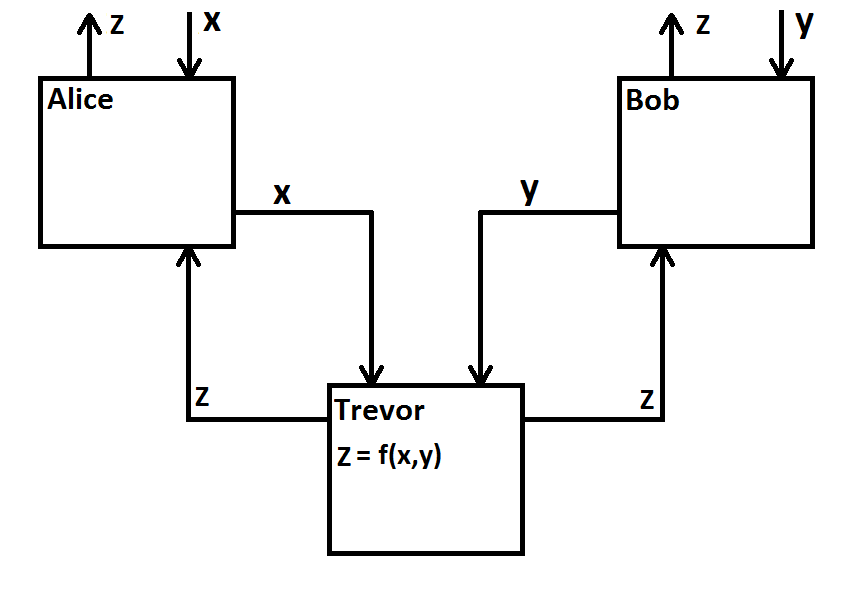
\includegraphics[scale=0.6]{Images/IdealModel}
		% Diagram. One big one will do me thinks.
	\end{frame}


	\begin{frame}
		\frametitle{Security Definitions}
		
		\begin{itemize}

		\item We measure the security of an SMC protocol in terms of what adversaries it is secure against, we define adversaries in terms of their capabilities.

		\item We say that an SMC protocl is secure against an adversary if the adversary can achieve no more than they would be able to achieve attacking the Ideal Model.

		\item We focus on three adversaries,
			\begin{itemize}
			\item Semi-Honest 
			\item Malicious 
			\item Covert
			\end{itemize}
		\end{itemize}
		% Acknowledge we're skipping over Static and Active corruption issues.

	\end{frame}
	\begin{frame}
		\frametitle{Security Definitions}
		
		\begin{itemize}

		\item We measure the security of an SMC protocol in terms of what adversaries it is secure against, we define adversaries in terms of their capabilities.

		\item We say that an SMC protocl is secure against an adversary if the adversary can achieve no more than they would be able to achieve attacking the Ideal Model.

		\item We focus on three adversaries,
			\begin{itemize}
				\item Semi-Honest 
				\item Malicious 
				\item Covert
			\end{itemize}
		\end{itemize}
		% Acknowledge we're skipping over Static and Active corruption issues.

	\end{frame}
	
	\begin{frame}
		\frametitle{Semi-Honest Adversaries}
		\begin{itemize}
			\item Semi-Honest(SH) adversaries are the weakest adversary we shall consider.
			\item They are sometimes also called ``honest, but curious''.
			\item SH adversaries are limited to looking at information given to them in the process of the protocol.
			\item They have to follow the protocol (they cannot cheat). 
			\item SH adversaries are very similar to traditional ``Passive'' adversaries.
		\end{itemize}
	\end{frame}

	\begin{frame}
		\frametitle{Malicious Adversaries}
		\begin{itemize}
			\item Malicious adversaries are the strongest adversary.
			\item Malicious adversaries can perform 
		\end{itemize}
	\end{frame}


	\begin{frame}
		\frametitle{Oblivious Transfer}
		A key component we will need later is Oblivious transfer(OT).\\
      
		\begin{figure}[!htb]
			%\begin{mdframed}
				\centering
				\begin{minipage}{0.45\textwidth}
					\centering
					\textbf{Receiver}\\
					Inputs : $b \in \{0, 1\}$\\
					Outputs : $X_b$\\
				\end{minipage}

				\begin{minipage}{0.45\textwidth}
					\centering
					\textbf{Sender}\\
					Inputs : $X_1$, $X_2$\\
					Outputs : $\emptyset$\\
				\end{minipage}

			%\end{mdframed}
			\caption{ Definition of the functionality of a one-out-of-two OT protocol.\label{fig:OTformalDef}}
		\end{figure}
		% Diagram really needed for this.

	\end{frame}


	\begin{frame}
		\frametitle{Security levels for OTs}
		
	\end{frame}



\end{document}
